\section{OT-Security}

\subsection{Abgrenzung IT-Security und OT-Security}

Die Unterscheidung zwischen IT-Security und OT-Security ist in der Sicherheitsarchitektur industrieller Systeme von zentraler Bedeutung. Während IT-Security hauptsächlich darauf abzielt, Informations- und Kommunikationstechnologien zu sichern, konzentriert sich OT-Security auf die Absicherung von Steuerungs- und Automatisierungstechnologien, die direkt physikalische Prozesse in industriellen Umgebungen beeinflussen. Mit OT meint es "[...] Hard- und Software, die physische Geräte, Prozesse und Ereignisse in der Institution überwacht und steuert" (\cite {ICS}, S. 9). Diese Unterschiede zeigen sich auch in der grundlegenden Denkweise: Während die IT virtuell ist, ist die OT physisch. Ein weiterer wesentlicher Unterschied liegt in den Schutzzielen, die unterschiedlich priorisiert werden. Gemäß des BSI sind die primären Schutzziele wie folgt definiert (vgl. \cite{BSI}): 
\begin{itemize}
\item \textbf{Vertraulichkeit}: Nur autorisierte Personen haben Zugriff zu den Informationen.
\item \textbf{Integrität}: Die Information wurde auf dem Transportweg nicht verändert.
\item \textbf{Verfügbarkeit}: Kommunikationsdienste stehen zu den gewünschten Zeitpunkten zur Verfügung.
\end{itemize}
Zusätzlich zu diesen Zielen spielt in der OT-Security auch das Schutzziel Safety eine bedeutende Rolle. Safety zielt darauf ab, Personen und die Umwelt vor physischen Schäden zu schützen, indem Maßnahmen ergriffen werden, um Unfälle zu verhindern oder ihre Auswirkungen zu minimieren (vgl. \cite{Safety}). Die unterschiedliche Hierarchie der Schutzziele wird in den folgenden Abbildungen veranschaulicht:
\begin{figure}[h]
    \centering
    \begin{minipage}{0.45\textwidth}
        \centering
        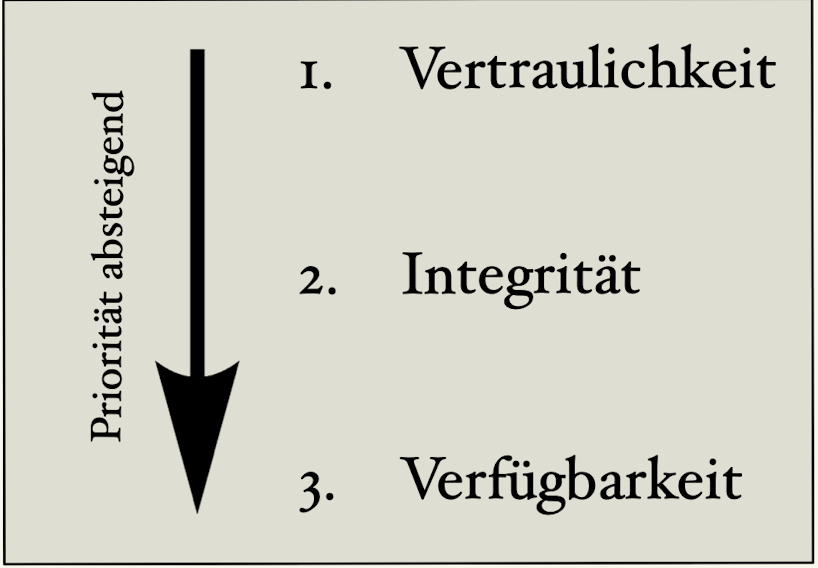
\includegraphics[scale=.3]{images/ITS.png}
        \caption{Schutzziele IT-Security}
        \label{fig:meine-grafik1}
    \end{minipage}
    \hfill
    \begin{minipage}{0.45\textwidth}
        \centering
        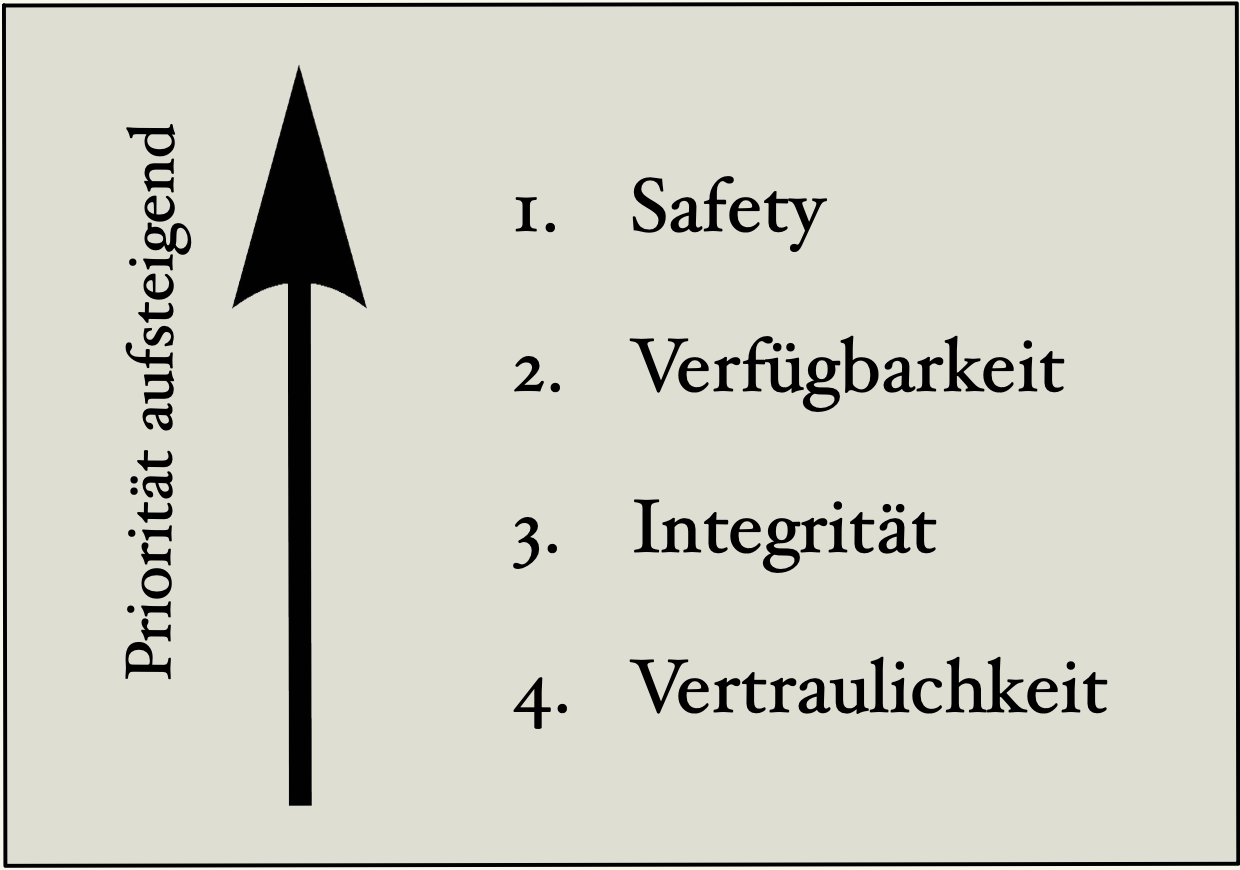
\includegraphics[scale=.299]{images/OTS.png}
        \caption{Schutzziele OT-Security}
        \label{fig:meine-grafik2}
    \end{minipage}
\end{figure}
\\ Konzeptionell verfolgen beide Ansätze verschiedene Rangordnungen der Schutzziele. Für die OT-Security ist die Verfügbarkeit industrieller Anlagen zu jedem Zeitpunkt von besonderer Bedeutung. Für Industriebetriebe ist dies essenziell, da ungeplante Ausfallzeiten im Schnitt 532.000 US-Dollar pro Stunde kosten (vgl. \cite{OTS/ITS}). 
\subsection{Herausforderungen und Bedrohungslage}

Das ICS Security Kompendium des BSI ist ein Grundlagenwerk, das Organisationen dabei unterstützt, Cybersicherheitsrisiken in der OT zu erkennen und zu bewältigen, indem es Basiswissen vermittelt, Maßnahmen und Prozesse beschreibt sowie Verbindungen zu relevanten Standards und Gesetzen herstellt. Hierbei werden drei grundsätzliche Schwachstellen im OT-Umfeld definiert. Man unterteilt in Organisatorische Schwachstellen, Technische Schwachstellen und die Schwachstelle Lieferkette. 

\subsubsection{Organisatorische Schwachstellen}

Die Sicherheit industrieller Steuerungssysteme (OT-Umgebungen) ist essenziell für die Aufrechterhaltung kritischer Infrastrukturen, aber oft durch diverse organisatorische Schwachstellen gefährdet. Eine zentrale Schwäche liegt in unzureichenden oder fehlenden organisatorischen Regelungen sowie einer mangelhaften Dokumentation zur Cybersicherheit. Diese bilden die Grundlage für effektive Entscheidungsfindung und Maßnahmen, und ihr Fehlen kann potenzielle Sicherheitslücken verursachen, die ausgenutzt werden könnten.
Ein weiteres kritisches Problem ist das unzureichende Risikomanagement in OT-Umgebungen. Ohne eine gründliche Identifikation und Bewertung potenzieller Gefahren können Schwachstellen und Bedrohungen übersehen oder falsch priorisiert werden, was zu ungeeigneten oder unzureichenden Schutzmaßnahmen führt. Dies wiederum könnte die Reaktionsfähigkeit auf Sicherheitsvorfälle beeinträchtigen und die Auswirkungen solcher Zwischenfälle verschlimmern. Ein bedeutender Aspekt ist auch die mangelnde Kommunikation innerhalb der Organisationen. Klar definierte Richtlinien und Verfahren müssen nicht nur vorhanden sein, sondern auch effektiv kommuniziert werden, um Missverständnisse zu vermeiden und sicherzustellen, dass Sicherheitsmaßnahmen korrekt umgesetzt werden. Eine unzureichende Dokumentation und Kommunikation können im Ernstfall zu erheblichen Verzögerungen bei der Fehlerdiagnose und -behebung führen, was die Ausfallzeiten und die Wiederherstellungszeiten erhöht. Ein weiteres Problem ergibt sich aus der Übertragung ungeeigneter IT-Praktiken auf das OT-Umfeld. Da IT- und OT-Systeme unterschiedliche Anforderungen und Betriebsabläufe haben, können Sicherheitsmaßnahmen und -standards aus der IT nicht einfach auf OT-Systeme übertragen werden. Dies kann zu inkonsistenten oder unzureichenden Sicherheitslösungen führen, die die spezifischen Risiken und Bedrohungen in OT-Umgebungen nicht angemessen berücksichtigen (vgl. \cite{ICS}, S. 31-34).

\subsubsection{Technische Schwachstellen}

In der Analyse der technischen Schwachstellen von OT-Systemen zeigt sich eine Vielzahl von Risiken, die durch unzureichende Sicherheitsmaßnahmen und veraltete Konfigurationen entstehen können. Ein zentraler Aspekt ist die unvollständige Absicherung von Fernzugängen, die autorisierten Personen ermöglichen, aus der Ferne auf Systeme zuzugreifen. Besonders relevant ist dies im Kontext zunehmender Nutzung von Homeoffice und mobilen Zugängen, jedoch sind diese Zugänge oft schlecht geschützt und können Angriffspunkte für Cyberkriminelle darstellen. Ein weiteres bedeutendes Risiko ergibt sich aus der fehlenden Überwachung der Infrastruktur, die dazu führen kann, dass sicherheitsrelevante Ereignisse und Schwachstellen nicht rechtzeitig erkannt werden. Dies birgt die Gefahr von Produktionsausfällen und Sicherheitsvorfällen, die erhebliche wirtschaftliche Schäden verursachen können. Zusätzlich sind OT-Netze zunehmend von IT-Netzen abhängig, was potenzielle Sicherheitslücken durch gemeinsam genutzte Infrastruktur und Dienste schafft. Störungen oder Angriffe in IT-Netzen können sich direkt auf OT-Umgebungen auswirken und zu schwerwiegenden Konsequenzen führen, wie z.B. Produktionsausfällen oder sogar Sicherheitsrisiken für Mensch und Umwelt. Ein weiteres kritisches Thema ist die Verwendung von Legacy-Systemen, die aufgrund ihrer veralteten Sicherheitsmechanismen und der fehlenden Herstellerunterstützung besonders anfällig für Cyberangriffe sind. Diese Systeme können moderne Sicherheitsbedrohungen oft nicht effektiv abwehren und stellen somit ein erhebliches Risiko für die Sicherheit von OT-Umgebungen dar (vgl. \cite{ICS}, S. 34-39). 


\subsubsection{Schwachstelle Lieferkette}

Die Lieferketten für industrielle Steuerungssysteme haben in den letzten Jahren verstärkt das Interesse von Cyberangreifern auf sich gezogen. Diese Angreifer nutzen gezielt Schwachstellen in der Lieferkette aus, um Schadsoftware oder Hintertüren in die OT-Komponenten einzuschleusen. Dadurch können sie unautorisierten Zugriff auf kritische Infrastrukturen wie Stromnetze, Wasserversorgung oder Verkehrssteuerungssysteme erlangen.
Ein zentraler Aspekt sind unzureichende Sicherheitsregelungen innerhalb der Lieferkette. Wenn die Verantwortlichkeiten für die Cybersicherheit nicht klar geregelt sind, entstehen Gefahrenpunkte, da niemand sich zuständig fühlt, potenzielle Schwachstellen zu identifizieren und zu beheben. Hardware-Hintertüren sind eine weitere schwerwiegende Schwachstelle. Diese ermöglichen es Herstellern oder Dritten, verdeckte Zugänge zu Systemen oder Daten einzurichten. Solche Hintertüren können durch das Hinzufügen von Schnittstellen oder speziellen Codes in die Firmware oder das BIOS der OT-Komponenten entstehen. Die Firmware, als entscheidendes Element für die Funktion der Steuergeräte, ist ebenfalls anfällig für Schwachstellen. Diese können durch fest einprogrammierte Zugangsdaten oder fehlerhafte Entwicklungspraktiken entstehen. Modifizierte Firmware, die während des Transports oder durch kompromittierte Updates eingespielt wird, ermöglicht es Angreifern, Geräte fernzusteuern oder sensible Daten auszulesen. Die Kryptographie, die zur Sicherung von Daten verwendet wird, ist nicht immun gegen Schwachstellen. Fehlerhafte Implementierungen oder veraltete Verfahren können es Angreifern erleichtern, verschlüsselte Daten zu entschlüsseln oder Manipulationen vorzunehmen. Neben der Firmware sind auch Anwendungssoftware und deren Integration in die IT-Infrastruktur potenzielle Einfallstore für Angreifer. Standard IT-Betriebssysteme wie Windows oder Linux, die für diese Anwendungen genutzt werden, sind selbst häufig Ziel von Cyberangriffen. Ein unsicherer Beschaffungsprozess, bei dem Cybersicherheitsanforderungen nicht ausreichend berücksichtigt werden, trägt ebenfalls zur Verwundbarkeit der Lieferkette bei. Ebenso können Fehler bei der Implementierung und Integration von Anlagenkomponenten durch verschiedene Hersteller Sicherheitslücken erzeugen, die ausgenutzt werden können. Externe Dienstleister, die unsichere Geräte oder ungeprüfte Zugriffe auf Anlagen verwenden, stellen ein weiteres Risiko dar. Ebenso birgt die Nutzung externer Plattformen und Cloud-Infrastrukturen Herausforderungen wie mangelnde Kontrolle über Sicherheitsmaßnahmen und potenzielle Schwachstellen bei der Datenübertragung (vgl. \cite{ICS}, S. 39-41).

\subsection{Maßnahmen}

Im Bereich der OT-Security (Operational Technology Security) sind gezielte Maßnahmen von entscheidender Bedeutung, um die Sicherheit und Integrität industrieller Steuerungssysteme zu gewährleisten. Die Implementierung spezifischer Schutzmechanismen ist notwendig, um sowohl unbefugte Zugriffe als auch potenzielle Cyberangriffe wirksam zu verhindern. Angreifer nutzen zunehmend fortschrittliche Werkzeuge, einschließlich Künstlicher Intelligenz, um ihre Angriffe zu verfeinern, weshalb ein kontinuierliches Update der Sicherheitstechnologien und -praktiken unerlässlich ist. Bei der Übertragung von IT-Sicherheitsmaßnahmen auf OT-Umgebungen ist zu berücksichtigen, dass nicht alle Maßnahmen problemlos übertragbar sind, da beispielsweise Schadsoftware-Scanner in Produktionsumgebungen zu Ausfällen führen können, was dem Schutzziel der Verfügbarkeit widerspricht.

Die Segmentierung von Netzwerken stellt eine bewährte Strategie dar, um die Netzwerksicherheit zu verbessern. Dieser Ansatz teilt ein größeres Netzwerk in kleinere, autonome Subnetze auf, was eine bessere Überwachung, Kontrolle des Datenverkehrs sowie eine optimierte Netzwerkleistung ermöglicht. Zudem erleichtert er die Identifikation und Behebung technischer Probleme und schränkt die Ausbreitung von Malware innerhalb des Netzwerks ein (vgl. \cite{Netzwerksegmentierung}).

Die Netzwerkzugangskontrolle (Network Access Control, NAC) regelt, wer Zugriff auf das Netzwerk erhält und in welchem Umfang. Dies geschieht durch Authentifizierung, Identifizierung von Benutzern und Geräten sowie entsprechende Zuordnung und Autorisierung der Kommunikationsverbindungen. Während NAC-Systeme in der IT weit verbreitet und einfach zu implementieren sind, stellen sie in der Operational Technology (OT) spezifische und komplexere Anforderungen dar. Eine fehlerhafte Zuordnung oder Abkopplung eines Geräts in der OT kann erhebliche Auswirkungen auf die Anlagenverfügbarkeit haben (vgl. \cite{NAC}).

Organisatorische Schutzmaßnahmen wie die Etablierung einer internen Sicherheitsorganisation mit klaren Zuständigkeiten, die Aufstellung eines Business Continuity Plans zur Bewältigung von Störungen und Produktionsausfällen, regelmäßige Awareness-Schulungen für alle Mitarbeiter sowie eine umfassende Dokumentation der Systeme und Anlagen sind unverzichtbar im OT-Bereich. Diese Maßnahmen bilden die Grundlage für ein robustes Sicherheitskonzept, das klare Sicherheitsrichtlinien und -prozesse festlegt, deren regelmäßige Überprüfung und Aktualisierung angesichts sich wandelnder Bedrohungsszenarien sicherstellt (vgl. \cite{orga}).

\subsection{Fallbeispiele}
\subsubsection{STUXNET}


Im Bereich der Cybersicherheit und kritischen Infrastrukturen markiert das Jahr 2010 einen bedeutenden Meilenstein durch das Auftreten des Stuxnet-Wurms. Diese hochentwickelte Schadsoftware wurde entdeckt, als sie erfolgreich Zugang zu einem wichtigen industriellen Steuerungssystem verschaffte, das Teil eines Urananreicherungsprogramms im Iran war (vgl. \cite{Stuxnet}, S. 1 ff.). Die Auswirkungen waren drastisch: Etwa 1000 Uranzentrifugen wurden schwer beschädigt, was eine umfangreiche und kostspielige Reparatur erforderlich machte. Neu daran war, dass Cyberattacken zuvor nur indirekt die Grenze zur physikalischen Welt überschritten hatten. Dies änderte sich mit Stuxnet, da industrielle Anlagen direkt gestoppt und zerstört wurden (vgl. \cite{Fraunhofer}, S. 12). Stuxnet war bahnbrechend, weil es als erste Schadsoftware bekannt wurde, die über USB-Laufwerke Zielgeräte infizierte. Darüber hinaus konnte sich der Wurm eigenständig aktualisieren, indem er Peer-to-Peer-Kommunikation\footnote{Teilnehmer direkt miteinander verknüpft mit gleichen Rechten} und Online-Verbindungen nutzte. Durch den Einsatz einer gestohlenen digitalen Signatur gelang es ihm, ein Rootkit\footnote{Softwarewerkzeuge, die ermöglichen zukünftige Anmeldevorgänge des Eindringlings zu verbergen sowie Prozesse und Dateien zu tarnen} zu installieren, was seine fortschrittlichen und zielgerichteten Angriffsmethoden verdeutlichte (vgl. \cite{NordVPN}).

\subsubsection{TRITON}

Der Vorfall mit TRISIS im Sommer 2017 markierte einen bedeutenden Zwischenfall im Bereich der kritischen Infrastrukturen, insbesondere in einem Chemiewerk in Saudi-Arabien. Ursprünglich als technischer Fehler in den Safety-Systemen des Herstellers Schneider Electric vermutet, stellten Sicherheitsexperten fest, dass dieser Vorfall auf eine gezielte Schadsoftware zurückzuführen war. Die Malware, bekannt als TRISIS, infiltrierte die TRICONEX Safety-Systeme, die für sicherheitsrelevante Aktionen in der Anlage zuständig sind, und hatte potenziell katastrophale Auswirkungen, wäre der Fehler nicht entdeckt worden. Der Angriff nutzte mehrere Schwachstellen aus, darunter einen offen zugänglichen Schlüsselschalter im Programmiermodus sowie unzureichende Netzwerksegmentierung, die den Angreifer Zugang zur Engineering-Station verschaffte. Diese Station wurde verwendet, um das Safety-System zu programmieren, und bot damit eine Eintrittspforte für die Schadsoftware. TRISIS wurde speziell für TRICONEX-Systeme entwickelt und zielte darauf ab, sicherheitsrelevante Prozesse zu manipulieren oder zu stören. Der Vorfall weist auf die Gefahr hin, dass auch hochsichere Safety-Systeme anfällig für digitale Angriffe sind, unabhängig von der Qualität oder Herkunft der verwendeten Software. Während keine unmittelbaren physischen Schäden gemeldet wurden, verdeutlicht dieser Vorfall die potenziellen Risiken staatlich finanzierter Cyberangriffe, die gezielt industrielle Steuerungssysteme ins Visier nehmen. Die komplexe Natur von TRISIS und seine spezifische Ausrichtung legen nahe, dass der Angriff möglicherweise für einen begrenzten Kreis entwickelt wurde, jedoch schwerwiegende Konsequenzen gehabt hätte, wenn er erfolgreich gewesen wäre. Für zukünftige Sicherheitsmaßnahmen wird empfohlen, Safety-Systeme strikt vom restlichen Automatisierungsnetzwerk abzuschotten oder sogar physisch zu isolieren. Maßnahmen wie Firewalls, Intrusion Detection Systeme und regelmäßige Bedrohungsanalysen sind entscheidend, um solche Angriffe frühzeitig zu erkennen und zu verhindern. Die Integration von Sicherheitsaspekten (Security-by-Design) in die Entwicklung von Safety-Systemen sowie die Einhaltung entsprechender Normen wie der IEC 62443 sind unerlässlich, um kritische Infrastrukturen vor zukünftigen Bedrohungen zu schützen. Diese Ereignisse unterstreichen die Notwendigkeit einer ganzheitlichen Sicherheitsstrategie in der zunehmend vernetzten Welt industrieller Netzwerke (vgl. \cite{TRISIS}).

